\lecture{1}{27. Januar 2025}{Introduction to Materials Science}

\section{Introduction to Materials Science}
\subsection{Historical perspective}
Materials development is a cornerstone in societal advancement. Many previous time-periods have even been classified based on the most ``advanced'' materials used in the period (think ``the Stone Age'', ``the Bronze Age'', ``the Iron Age'' and so on).

\begin{dis}[What (material) age are we living in now?] %todo: make into discussion instead of example
  The by-far most prominent and tone-setting material in the current age is \textit{plastics}. For this reason we believe the most correct name for the current material age is ``the Plastic Age''.

  Other answers include: \textit{the Composite Age}, \textit{still the Iron Age}, \textit{the Composite age}, \textit{the Lithium Age}, \textit{the Bio-materials Age}, \textit{the Concrete Age}, \textit{the Titanium Age}, \textit{the Silicon Age}, or \textit{the Carbon Age}. Michal Budzik seems to agree the most with the \textit{the Plastics Age} or \textit{the Silicon Age}.
\end{dis}


\subsection{Materials Science and engineering}
It is important to note the small difference between \textit{Materials Science} and \textit{Materials Engineering}, both of which will be taught about during the course.

\begin{definition}[Materials Science]
  Materials Science seeks to investigate relationships between structures and properties of materials with the goal of designing or developing new materials.
\end{definition}

\begin{definition}[Materials Engineering]
  Materials Engineering seeks to create new product from existing materials with the goal of developing materials processing techniques among other things.
\end{definition}


\subsection{Classification and properties of materials}
We normally divide materials into 4 different categories:
\begin{enumerate}
  \item Metals
  \item Ceramics
  \item Polymers
  \item Composites
\end{enumerate}

In general the densities of the four classes are arranged as follows: $\rho_m > \rho_{cer} > \rho_p > \rho_{com}$ whereas for stiffness the ranking is more like $Y_m = Y_{cer} \geq Y_{com} > Y_p$.

\subsection{Materials selection and Ashby diagrams}

\subsubsection{Ashby Diagrams}

\begin{figure} [ht]
  \centering
  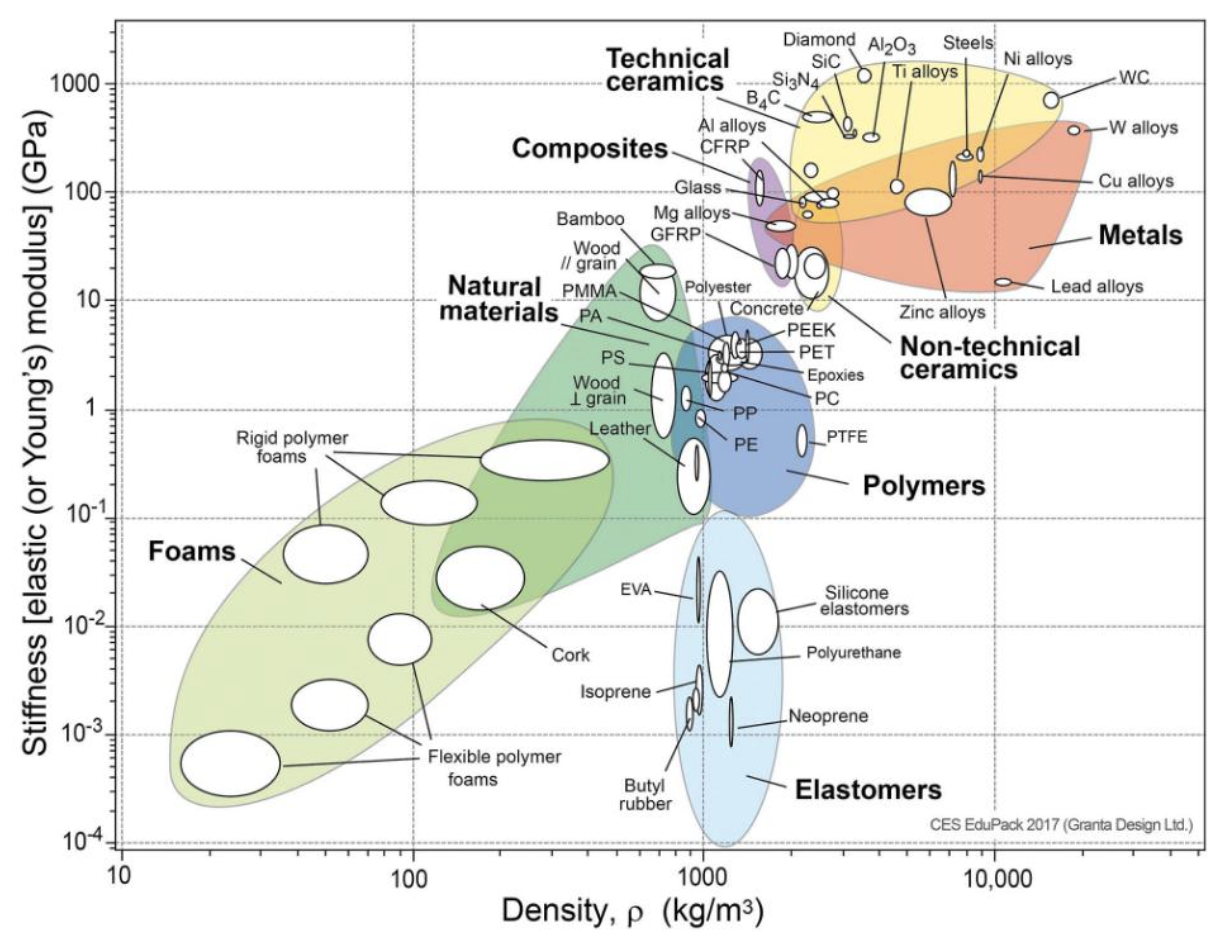
\includegraphics[width=0.65\linewidth]{./figures/F1_1.png}
  \caption{Ashby diagram for stiffness and density}
  \label{fig:F1_1}
\end{figure}
To better be able to get an understanding of how different materials differ in terms of two (or more factors) these factors can be plotted on a log-log-scale -- This is called an Ashby diagram. On \autoref{fig:F1_1} an Ashby diagram comparing stiffness and density is shown.

The properties of materials fall into the following 6 different general categories. These are:
\begin{itemize}
  \item Mechanical
  \item Electrical
  \item Thermal
  \item Magnetic
  \item Optical
  \item Deterioative
\end{itemize}

\subsubsection{Materials selection}
Whenever one has to select a material to use for a specific application one should stick to the following procedure.
\begin{enumerate}
  \item First of all one needs to understand the application the material will be used in. This helps determine which material properties are important.
  \item When the list of important properties have been made one needs to compare this list with known materials and see which aligns the best with the desired property.
  \item When the best candidate-material has been found one can start to investigate the best way to process the material to bring out the desired qualities to the fullest. 
\end{enumerate}
